\section{Chain Complexes}
\label{sec:Chain Complexes}
\begin{definition}
	A \emph{(non-negative) chain complex} $C$ is a collection of abelian groups $C_n$ together with group homomorphisms $\del_n: C_n \to C_{n-1}$, which we call \emph{boundary homomorphisms}, such that $\del_n \circ \del_{n+1} = 0$ for all $n \in \Np$.
\end{definition}

Thus graphically a chain complex $C$ can be depicted by the following diagram:
\begin{center}
\begin{tikzpicture}
	\matrix (m) [matrix of math nodes]{
		\cdots & C_4 & C_3 & C_2  & C_1 & C_0 \\
	};
	\foreach \d/\i/\j in {5/1/2,4/2/3,3/3/4,2/4/5,1/5/6} \path[->] (m-1-\i) edge node[auto] {$ \del_\d $} (m-1-\j);
\end{tikzpicture}
\end{center}

There are many variants to this notion. For example, there are also unbounded chain complexes with an abelian group for each $n \in \Z$ instead of $\N$. In this thesis we will only need chain complexes in the sense of the definition above. Hence we will simply call them chain complexes, instead of non-negative chain complexes. Other variants can be given by taking a collection of $R$-modules instead of abelian groups. Of course not any kind of mathematical object will suffice, because we need to be able to express $\del_n \circ \del_{n+1} = 0$, so we need some kind of \emph{zero object}. We will not need this kind of generality and stick to abelian groups.

In order to organize these chain complexes in a category, we should define what the maps are. The diagram above already gives an idea for this.
\begin{definition}
	Let $C$ and $D$ be chain complexes, with boundary maps $\del^C_n$ and $\del^D_n$ respectively. A \emph{chain map} $f: C \to D$ consists of a family of maps $f_n: C_n \to D_n$, such that they commute with the boundary operators: $f_n \circ \del^C_{n+1} = \del^D_{n+1} \circ f_{n+1}$ for all $n \in \N$, i.e. the following diagram commutes:
	\begin{center}
	\begin{tikzpicture}
		\matrix (m) [matrix of math nodes]{
			\cdots & C_4 & C_3 & C_2  & C_1 & C_0 \\
			\cdots & D_4 & D_3 & D_2  & D_1 & D_0 \\
		};
		\foreach \d/\i/\j in {5/1/2,4/2/3,3/3/4,2/4/5,1/5/6} \path[->] (m-1-\i) edge node[auto] {$ \del^C_\d $} (m-1-\j);
		\foreach \d/\i/\j in {5/1/2,4/2/3,3/3/4,2/4/5,1/5/6} \path[->] (m-2-\i) edge node[auto] {$ \del^D_\d $} (m-2-\j);
		\foreach \d/\i in {4/2,3/3,2/4,1/5,0/6} \path[->] (m-1-\i) edge node[auto] {$ f_\d $} (m-2-\i);
	\end{tikzpicture}
	\end{center}
\end{definition}

Note that if we have two such chain maps $f:C \to D$ and $g:D \to E$, then the levelwise composition will give us a chain map $g \circ f: C \to D$. Also taking the identity function in each degree, gives us a chain map $\id : C \to C$. In fact, this will form a category, we will leave the details (the identity law and associativity) to the reader.

\begin{definition}
	$\Ch{\Ab}$ is the category of chain complexes with chain maps.
\end{definition}

Note that we will often drop the indices of the boundary morphisms, since it is often clear in which degree we are working. The boundary operators give rise to certain subgroups, because all groups are abelian, subgroups are normal subgroups.

\begin{definition}
	Given a chain complex $C$ we define the following subgroups:
	\begin{itemize}
		\item $Z_n(C) = \ker(\del_n: C_n \to C_{n-1}) \nsubgrp C_n$, and
		\item $Z_0(C) = C_0$, and
		\item $B_n(C) = \im(\del_{n+1}: C_{n+1} \to C_n) \nsubgrp C_n$.
	\end{itemize}
\end{definition}
\begin{lemma}
	Given a chain complex $C$ we have for all $n \in \N$:
	$$ B_n(C) \nsubgrp Z_n(C).$$
\end{lemma}
\begin{proof}
	It follows from $\del_n \circ \del_{n+1} = 0$ that $\im(\del: C_{n+1} \to C_n)$ is a subset of $\ker(\del: C_n \to C_{n-1})$. Those are exactly the abelian groups $B_n(C)$ and $Z_n(C)$, so $ B_n(C) \nsubgrp Z_n(C) $.
\end{proof}
\begin{definition}
	Given a chain complex $C$ we define the \emph{$n$-th homology group} $H_n(C)$ for each $n \in \N$ as:
	$$ H_n(C) = Z_n(C) / B_n(C).$$
\end{definition}
\begin{lemma}
	The $n$-th homology group gives a functor $H_n : \Ch{\Ab} \to \Ab$ for each $n \in \N$.
\end{lemma}
\begin{proof}
	Let $f: C \to D$ be a chain map and $n \in \N$. First note that for $x \in Z_n(X)$ we have $\del^C(x) = 0$, so $\del^D(f_n(x)) = 0$, because the square on the right commutes:

	{\centering
	\begin{tikzpicture}
		\matrix (m) [matrix of math nodes, row sep=2em, column sep=2em]{
			\cdots & C_{n+1} & C_n & C_{n-1} & \cdots \\
			\cdots & D_{n+1} & D_n & D_{n-1} & \cdots \\
		};
		\foreach \i/\j in {1/2,2/3,3/4,4/5} \path[->] (m-1-\i) edge node[auto] {$ \del^C $} (m-1-\j);
		\foreach \i/\j in {1/2,2/3,3/4,4/5} \path[->] (m-2-\i) edge node[auto] {$ \del^D $} (m-2-\j);
		\path[->] (m-1-2) edge node[auto] {$ f_{n+1} $} (m-2-2);
		\path[->] (m-1-3) edge node[auto] {$ f_n $} (m-2-3);
		\path[->] (m-1-4) edge node[auto] {$ f_{n-1} $} (m-2-4);
	\end{tikzpicture}\par}

	So there is an induced group homomorphism $f^Z_n : Z_n(C) \to Z_n(D)$ (for $n=0$ this is trivial). Similarly there is an induced group homomorphism $f^B_n : B_n(C) \to B_n(D)$ by considering the square on the left. Now define the map $H_n(f) : x \mapsto [f_n(x)]$ for $x \in Z_n(C)$, we now know that $f_n(x)$ is also a cycle, because of $f^Z_n$. Furthermore it is well-defined on classes, because of $f^B_n$. So indeed there is an induced group homomorphism $H_n(f) : H_n(C) \to H_n(D)$.

	It remains to check that $H_n$ preserves identities and compositions. By writing out the definition we see $H_n(\id)([x]) = [\id(x)] = [x] = \id[x]$, and:
	$$ H_n(f \circ g)([x]) = [f_n(g_n(x))] = H_n(f)([g_n(x)]) = H_n(f) \circ H_n(g) ([x]). $$
\end{proof}

\todo{CC: What to do with the example...}
\subsection{The singular chain complex}
In order to see why we are interested in the construction of homology groups, we will look at an example from algebraic topology. We will see that homology gives a nice invariant for spaces. So we will form a chain complex from a topological space $X$. In order to do so, we first need some more notions.
\begin{definition}
	The topological space $\Delta^n$ is called the \emph{topological $n$-simplex} and is defined as:
	$$ \Delta^n = \{(x_0, x_1, \ldots, x_n) \in \R^{n+1} \I x_i \geq 0 \text{ and } x_0 + \ldots + x_n = 1 \}.$$
	The topology on $\Delta^n$ is the subspace topology.
\end{definition}

In particular $\Delta^0$ is simply a point, $\Delta^1$ a line and $\Delta^2$ a triangle. There are nice inclusions $\Delta^n \mono \Delta^{n+1}$ which we need later on. For any $n \in \N$ we define:
\begin{definition}
	For $i \in \{0, \ldots, n+1\}$ the $i$-th face map $\delta^i : \Delta^n \mono \Delta^{n+1}$ is defined as:
	$$ \delta^i (x_0, \ldots, x_n) = (x_0, \ldots, x_{i}, 0, x_{i+1}, \ldots, x_n) \text{ for all } x \in \Delta^n.$$
\end{definition}

For any space $X$, we will be interested in continuous maps $\sigma : \Delta^n \to X$, such a map is called a $n$-simplex. Note that if we have any continuous map $\sigma : \Delta^{n+1} \to X$ we can precompose with a face map to get $\sigma \circ \delta^i : \Delta^n \to X$, as shown in figure~\ref{fig:diagram_d}. This will be used for defining the boundary operator. We can make pictures of this, and when concerning continuous maps $\sigma : \Delta^{n+1} \to X$ we will draw the images in the space $X$, instead of functions.

\begin{figure}
	\begin{tikzpicture}
		\matrix (m) [matrix of math nodes]{
			\Delta^{n+1} & X \\
			\Delta^n & \\
		};
		\path[->]
		(m-1-1) edge node[auto] {$ \sigma $} (m-1-2)
		(m-2-1) edge node[auto] {$ \delta^i $} (m-1-1)
		(m-2-1) edge node[auto] {$ $} (m-1-2);
	\end{tikzpicture}
	\caption{The $(n+1)$-simplex $\sigma$ can be made into a $n$-simplex $\sigma \circ \delta^i$}
	\label{fig:diagram_d}
\end{figure}

\todo{Ch: Make some pictures here}

We now have enough tools to define the singular chain complex of a space $X$.

\begin{definition}
	For a topological space $X$ we define the \emph{$n$-th singular chain group} $C_n(X)$ as follows.
	$$ C_n(X) = \Z[\Hom{\cat{Top}}{\Delta^n}{X}] $$
	The boundary operator $\del : C_{n+1}(X) \to C_n(X)$ is defined on generators as:
	$$ \del(\sigma) = \sigma \circ \delta^0 - \sigma \circ \delta^1 + \ldots + (-1)^{n+1} \sigma \circ \delta^{n+1}.$$
\end{definition}

This might seem a bit complicated, but we can pictures this in an intuitive way, as in figure~\ref{fig:singular_chaincomplex}. And we see that the boundary operators really give the boundary of an $n$-simplex. To see that this indeed is a chain complex we have to proof that the composition of two such operators is the zero map.
\begin{figure}[h!]
	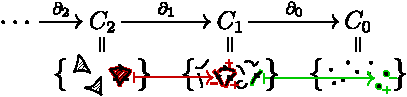
\includegraphics[scale=1.2]{singular_chaincomplex}
	\caption{The boundary of a 2-simplex, and a boundary of a 1-simple}
	\label{fig:singular_chaincomplex}
\end{figure}
\todo{CC: update picture}

\todo{Ch: Proposition: $C(X) \in \Ch{\cat{Ab}}$}
\todo{Ch: Example homology of some space}
\todo{Ch: Show that $\Ch{\Ab}$ is an ab. cat. At least show functoriality $\Hom{\Ch{\Ab}}{-}{-}$}
